\begin{figure}[htb]
    \centering
    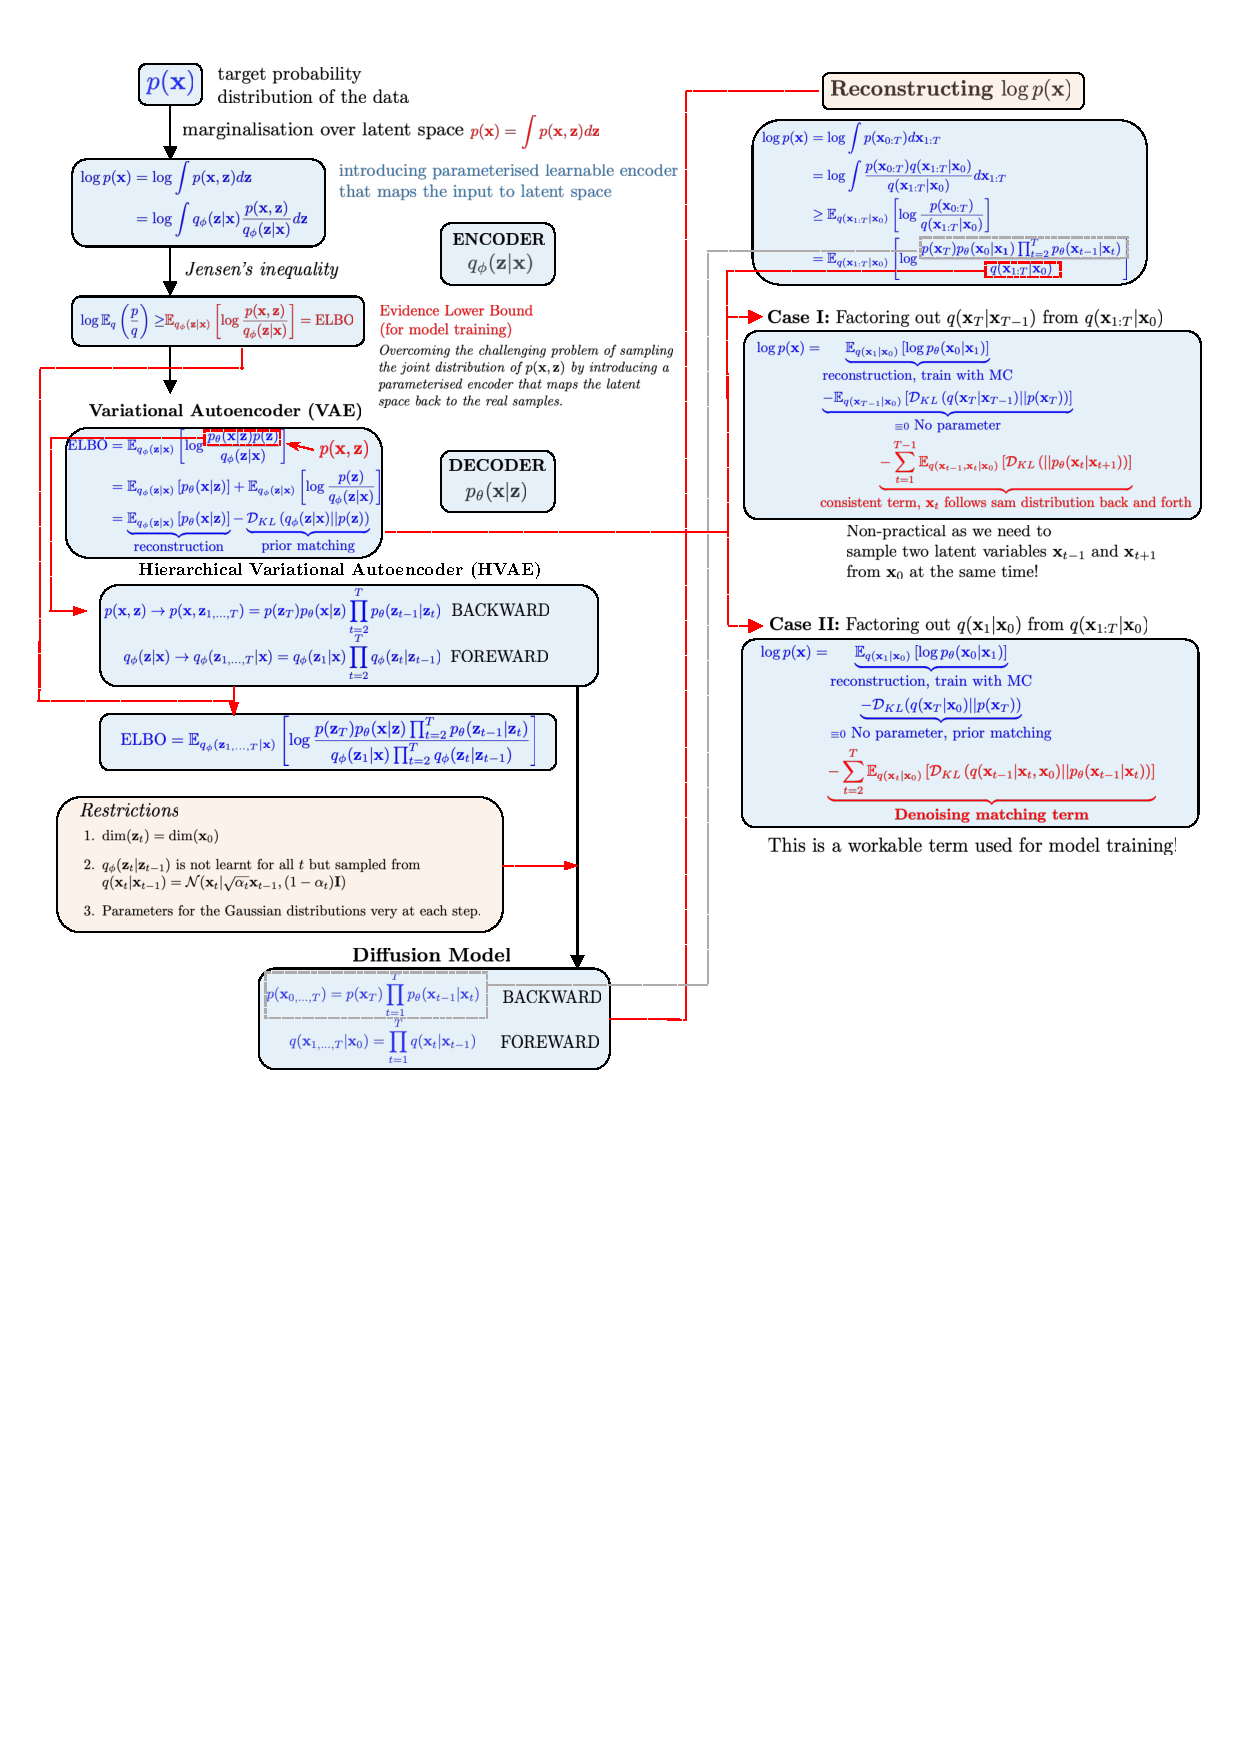
\includegraphics[width=\linewidth]{generative_model_relations.pdf}
    \caption{Relationship between variational autoencoder and the diffusion generative model, that is bridged via the hierarchical variational autoencoder, showcasing the key mathematical equations that are used to reconstruct the probability distribution of the target data $p(\bm{x})$, which are discussed in details by \citet{luo2022understanding}. Different variants and interpretations of the denoising term, that is used for training the diffusion generative models are further showcased in \cref{fig:denosing_process}.}
    \label{fig:generative_model_relations}
\end{figure}

\begin{figure}[htb]
    \centering
    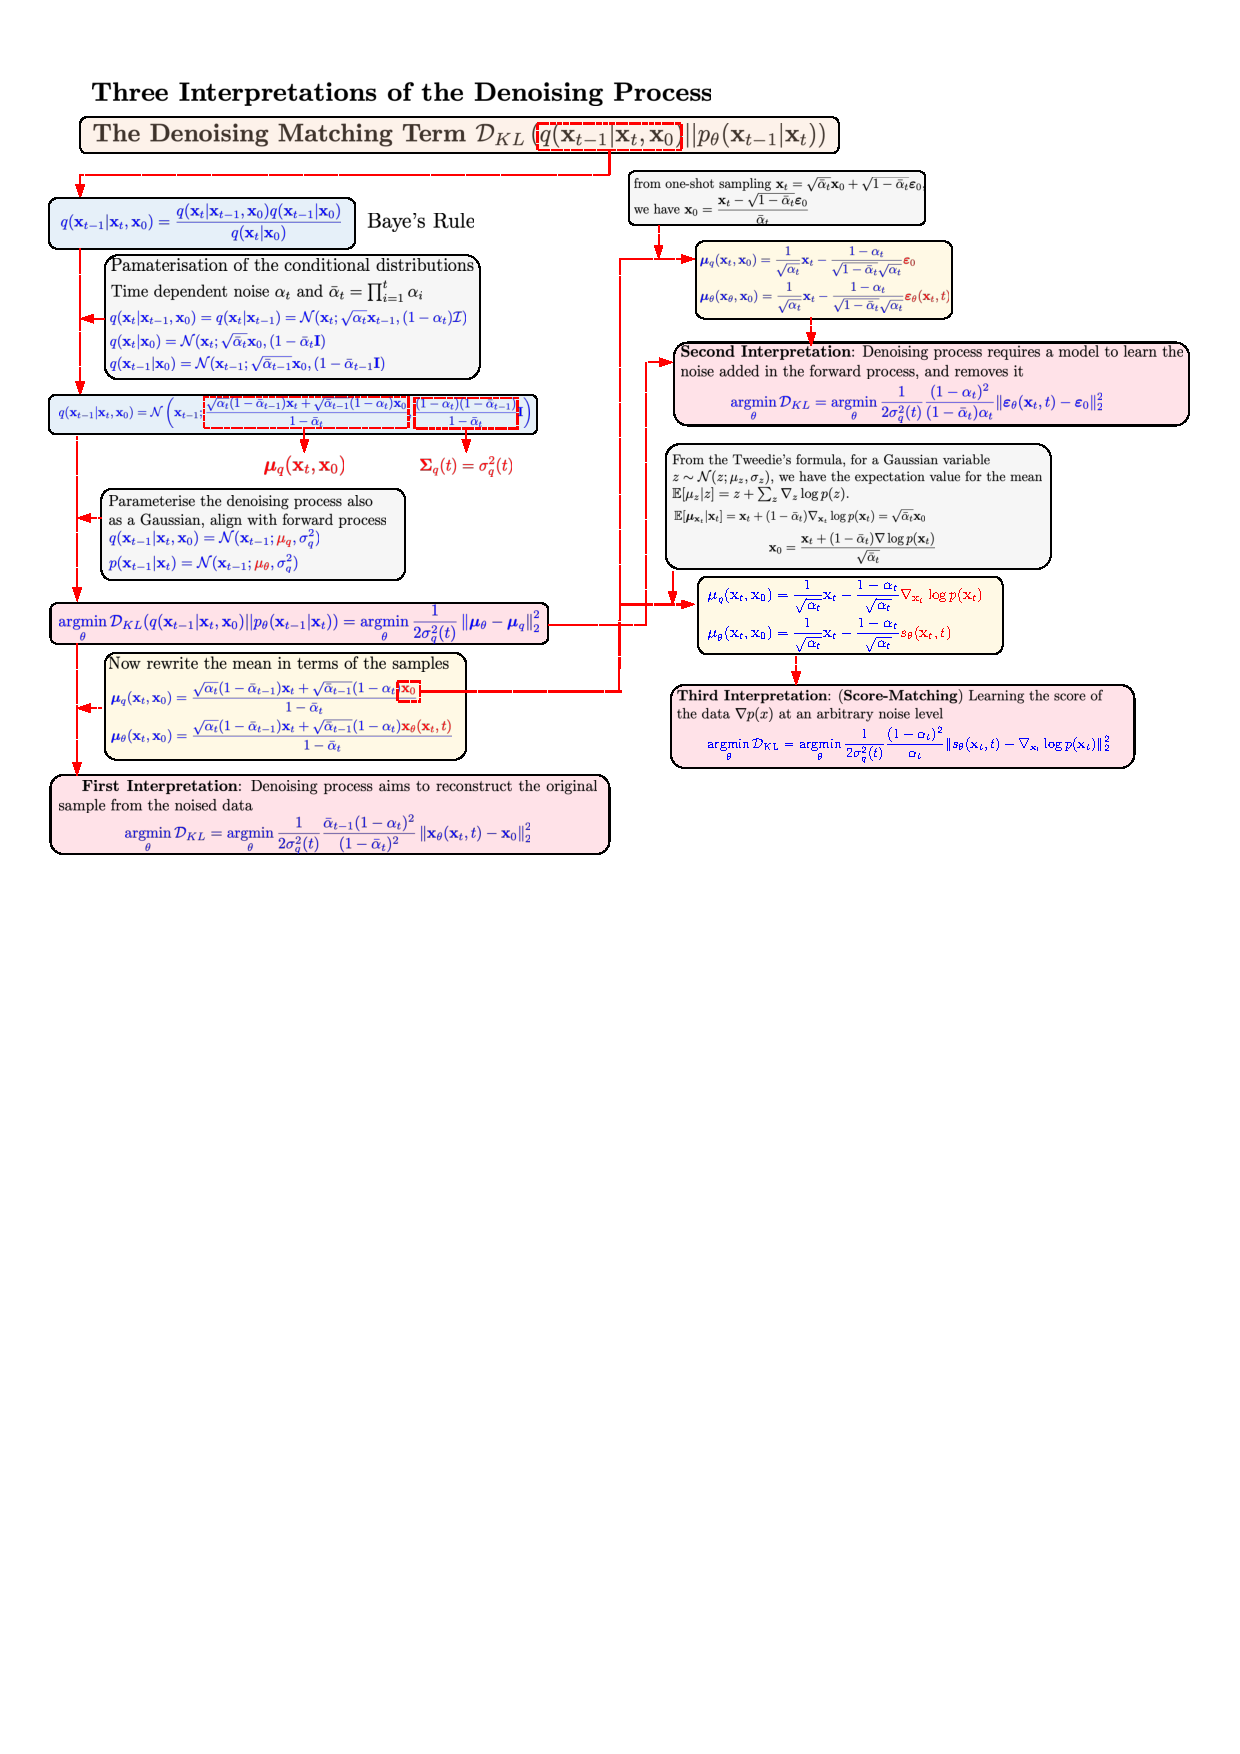
\includegraphics[width=\linewidth]{denosing_process.pdf}
    \caption{Relationship amongst three different ways to parameterise the transition probability in the reverse generative process for the diffusion generative model, from which computable expressions for the KL divergence between the forward and reverse process can be derived and interpreted for model training.}
    \label{fig:denosing_process}
\end{figure}